\documentclass{beamer}
\usetheme{Madrid}

\usepackage{graphicx}
\usepackage{hyperref}

\title{Fusion-JEPA Text-to-Speech}
\subtitle{Week 7 Progress Report}
\author{Omar Alkhammash \and Abdulrahman Soliman \and Hassan Alahmed}
\date{August 11, 2026}

\begin{document}

\begin{frame}
\titlepage
\end{frame}

\begin{frame}{Audio Generation Progress}
    \begin{itemize}
        \item \textbf{Significant Improvements:} We achieved noticeably better generation results over the last two weeks of continuous training.
        \item \textbf{Audio Output:} The SpatialDiT diffuser is finally outputting coherent audio waveforms. 
        \item \textbf{Acoustic Quality:} The generated samples sound distinctly like English speech, though the prosody and clarity are not quite perfect yet.
    \end{itemize}
    \begin{figure}
        \centering
        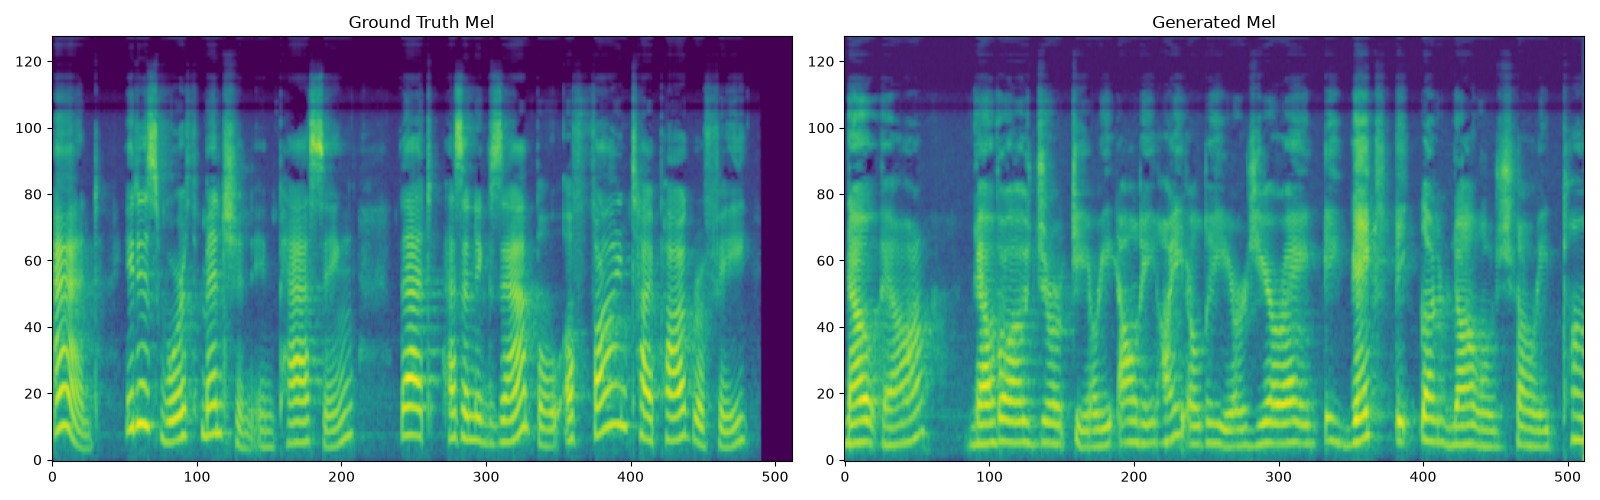
\includegraphics[width=0.9\textwidth,height=0.45\textheight,keepaspectratio]{images/output.jpg}
        \caption{Recent audio generation output showing strong structural foundations.}
    \end{figure}
\end{frame}

\begin{frame}{Architectural Enhancements}
    To achieve these results, we implemented several major changes to the model architecture:
    \begin{itemize}
        \item \textbf{Single-Stream Architecture:} We completely removed the Cross-Attention mechanism. Phoneme text embeddings are now concatenated directly to the visual tokens, forcing the model to process them in a unified single stream.
        \item \textbf{Removed Mean-Pooling:} We eliminated the mean-pooling layers to preserve the sequential alignment of phonemes, fixing the temporal destruction bottleneck.
        \item \textbf{Cosine Annealing:} Replaced static learning rates with a Cosine Annealing LR Scheduler to ensure smooth decay and convergence.
        \item \textbf{Targeted Freezing:} We introduced a training mechanism to completely freeze the SpatialDiT diffuser, allowing the JEPA backbone to learn mapping exclusively.
    \end{itemize}
\end{frame}

\begin{frame}{Current Training Status}
    \begin{itemize}
        \item \textbf{JEPA Backbone Training:} As we speak, the model is actively training the JEPA backbone while the diffuser remains strictly frozen.
        \item \textbf{Cloud Sync:} The training pipeline is fully automated and is uploading checkpoints directly to Hugging Face in real-time.
    \end{itemize}
    \vspace{0.2cm}
    \begin{figure}
        \centering
        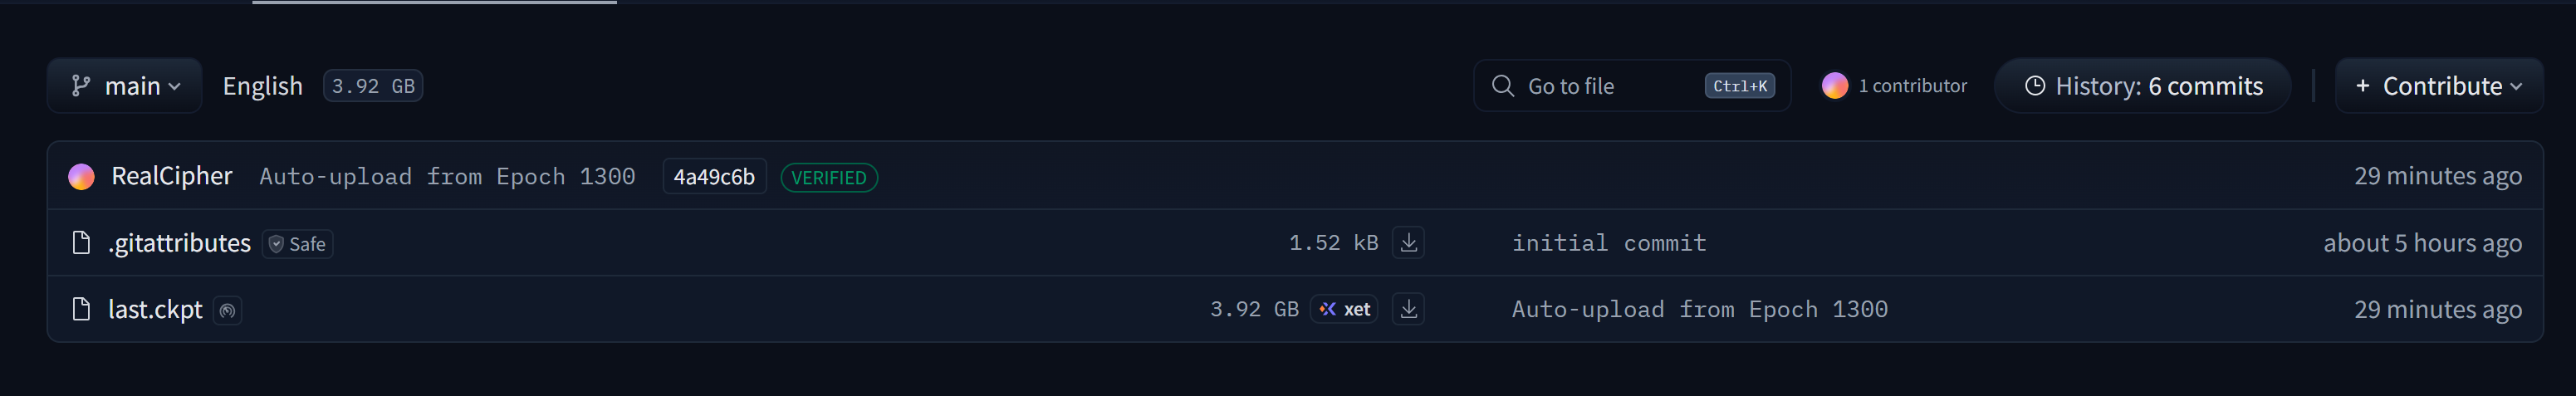
\includegraphics[width=0.9\textwidth]{images/screenshot.png}
        \caption{Live training logs and Hugging Face checkpoint uploads.}
    \end{figure}
\end{frame}

\begin{frame}{Future Work \& Next Steps}
    \begin{itemize}
        \item \textbf{Diffuser Fine-Tuning:} Once the JEPA backbone has fully converged and learned robust text-to-spectrogram mappings, we will unfreeze the SpatialDiT diffuser. The diffuser will then be fine-tuned on the significantly better structural inputs provided by the JEPA.
        \item \textbf{Arabic Model Training:} Following the successful optimization and training of the English model pipeline, we will initiate training for the Arabic model utilizing the exact same single-stream architecture.
    \end{itemize}
\end{frame}

\end{document}
